A Convolutional Neural Network (ConvNet/CNN) is a Deep Learning algorithm that can take in an input image, assign importance (learnable weights and biases) to various aspects/objects in the image, and be able to differentiate one from the other. The pre-processing required in a ConvNet is much lower as compared to other classification algorithms. While in primitive methods filters are hand-engineered, with enough training, ConvNets have the ability to learn these filters/characteristics.
\\ \\
The architecture of a ConvNet is analogous to that of the connectivity pattern of Neurons in the Human Brain and was inspired by the organization of the Visual Cortex. Individual neurons respond to stimuli only in a restricted region of the visual field known as the Receptive Field. A collection of such fields overlap to cover the entire visual area.
\\ \\
The Convolutional Neural Networks enable machines to view the world as humans do, perceive it in a similar manner and even use the knowledge for a multitude of tasks such as Image $\&$ Video recognition, Image Analysis $\&$ Classification, Media Recreation, Recommendation Systems, Natural Language Processing, etc. 

\begin{figure}[h]
    \centering
    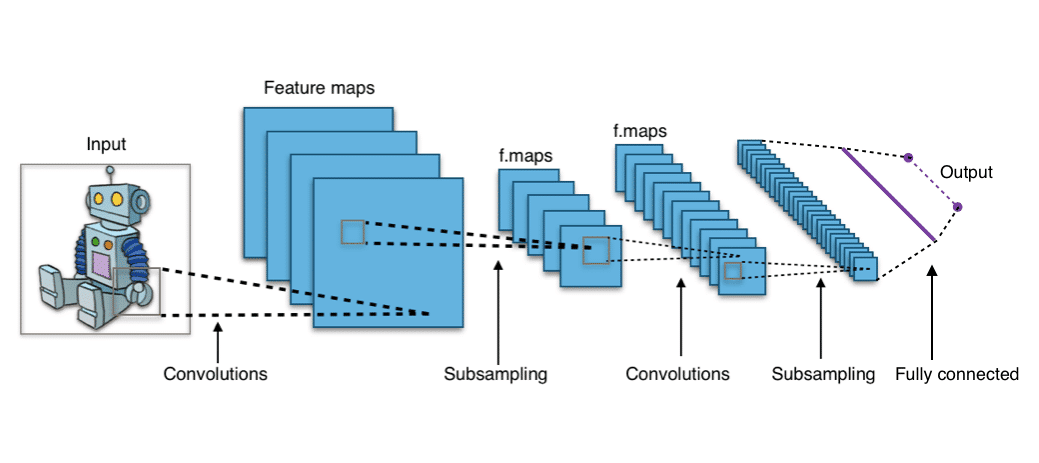
\includegraphics[scale=0.4]{CNN4.png}
    \caption{Convolutional Neural Network}
\end{figure}

\section{CNNs vs Feed-forward Neural Nets!}
    An image is nothing but a matrix of pixel values, right? So why not just flatten the image (e.g. 3x3 image matrix into a 9x1 vector) and feed it to a Multi-Level Perceptron for classification purposes?
\\ \\
    In cases of extremely basic binary images, the method might show an average precision score while performing prediction of classes but would have little to no accuracy when it comes to complex images having pixel dependencies throughout.
\\ \\
    A ConvNet is able to successfully capture the Spatial and Temporal dependencies in an image through the application of relevant filters. The architecture performs a better fitting to the image dataset due to the reduction in the number of parameters involved and the reusability of weights. In other words, the network can be trained to understand the sophistication of the image better.

\section{Convolution Layer — The Kernel}
    Each convolutional layer contains a series of filters known as convolutional kernels. The filter is a matrix of integers that are used on a subset of the input pixel values, the same size as the kernel. Each pixel is multiplied by the corresponding value in the kernel, then the result is summed up for a single value for simplicity representing a grid cell, like a pixel, in the output channel/feature map. These are linear transformations, each convolution is a type of affine function.

    \begin{figure}[h]
        \centering
        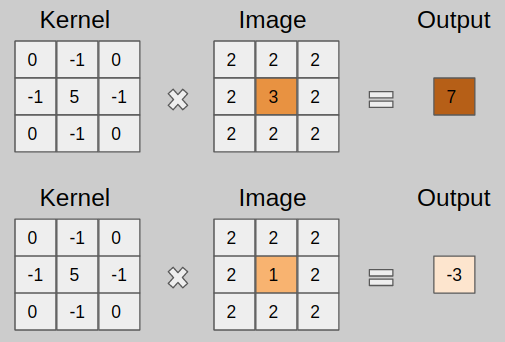
\includegraphics[scale=0.4]{CNN3.png}
        \caption{Average and Max pooling layer}
    \end{figure}

    In computer vision, the input is often a 3 channel RGB image. For simplicity, if we take a greyscale image that has one channel (a two-dimensional matrix) and a 3x3 convolutional kernel (a two-dimensional matrix). The kernel strides over the input matrix of numbers moving horizontally column by column, sliding/scanning over the first rows in the matrix containing the images pixel values. Then the kernel strides down vertically to subsequent rows. Note, the filter may stride over one or several pixels at a time, this is detailed further below. In other non-vision applications, a one-dimensional convolution may slide vertically over an input matrix.

\section{Pooling Layer}
    Similar to the Convolutional Layer, the Pooling layer is responsible for reducing the spatial size of the Convolved Feature. This is to decrease the computational power required to process the data through dimensionality reduction. Furthermore, it is useful for extracting dominant features that are rotational and positional invariant, thus maintaining the process of effectively training of the model.
\\ \\
    There are two types of Pooling: Max Pooling and Average Pooling. Max Pooling returns the maximum value from the portion of the image covered by the Kernel. On the other hand, Average Pooling returns the average of all the values from the portion of the image covered by the Kernel.

    \begin{figure}[h]
        \centering
        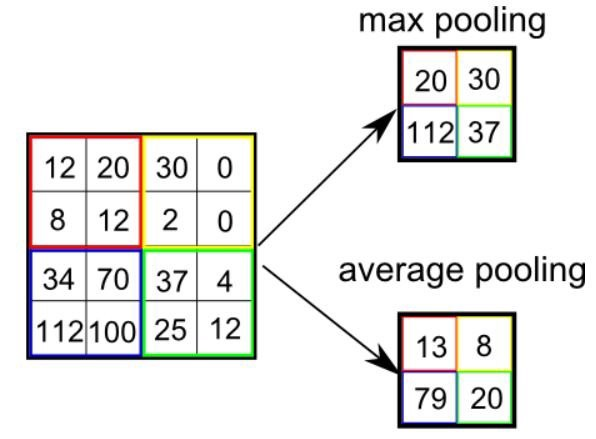
\includegraphics[scale=0.4]{CNN1.jpeg}
        \caption{Average and Max pooling layer}
    \end{figure}

    Max Pooling also performs as a Noise Suppressant. It discards the noisy activations altogether and also performs de-noising along with dimensionality reduction. On the other hand, Average Pooling simply performs dimensionality reduction as a noise suppressing mechanism. Hence, we can say that Max Pooling performs a lot better than Average Pooling.
\\ \\
    The Convolutional Layer and the Pooling Layer, together form the i-th layer of a Convolutional Neural Network. Depending on the complexities in the images, the number of such layers may be increased for capturing low-levels details even further, but at the cost of more computational power.
\\ \\
    After going through the above process, we have successfully enabled the model to understand the features. Moving on, we are going to flatten the final output and feed it to a regular Neural Network for classification purposes.
